\section{Bounding a relaxation by computer}\label{sec:method}

For more than one angle on each side we do not know how to evaluate $G(A;B)$ by hand, so we bound it by computer. The method is that of Kallus and Romik \cite[Sections~2--3]{kallusromik2018}, with two changes: some hallways are mirrored, and the search for a proof, done in floating-point arithmetic, is separated from its verification, done in exact arithmetic.

Throughout this section $A$ and $B$ are finite subsets of $(0\dg,90\dg)$, not both empty, and we list the $k=|A|+|B|$ hallways as $X_1,\dots,X_k$. For a hallway $L_a(\bu)$ we put $f_j=f_a$ and $g_j=g_a$, and for a mirrored hallway $\rho(L_b(\bv))$ we put $f_j=f_b\circ\rho$ and $g_j=g_b\circ\rho$. Since $\rho$ is its own inverse, in both cases
\begin{equation}\label{eq:Xj}
X_j(\bu)=\{u_1\le f_j\le u_1+1,\ g_j\le u_2+1\}\cup\{f_j\le u_1+1,\ u_2\le g_j\le u_2+1\},
\end{equation}
where $f_j$ and $g_j$ are affine functions and $\bu=(u_1,u_2)\in\R^2$ is the translation parameter of the $j$-th hallway. A point $\bw=(\bu^{(1)},\dots,\bu^{(k)})\in\R^{2k}$ collects all parameters, and we write $X(\bw)=\bigcap_{j}X_j(\bu^{(j)})$. Then $G(A;B)=\sup_{\bw}\lamstar\big(H\cap X(\bw)\big)$.


\subsection{A compact parameter box}

The supremum in the definition of $G(A;B)$ runs over all of $\R^{2k}$. The first step is to restrict it to an explicit box.

\begin{lem}[Normalisation]\label{lem:box}
Let $W\ge\min_{a\in A\cup B}W_a$, where $W_a$ is as in \cref{lem:width}, and let $B_W=[0,W]\times[0,1]$. For each $j$ let
\[
I_j=\big[\min_{B_W}f_j-1,\ \max_{B_W}f_j\big], \qquad J_j=\big[\min_{B_W}g_j-1,\ \max_{B_W}g_j\big],
\]
and let $E_0=\prod_{j=1}^k(I_j\times J_j)\subset\R^{2k}$. Then
\[
G(A;B)=\sup_{\bw\in E_0}\lamstar\big(B_W\cap X(\bw)\big).
\]
\end{lem}

\begin{proof}
Since $B_W\subset H$, the right-hand side is at most $G(A;B)$. For the converse, let $\bw\in\R^{2k}$ and let $K$ be a connected component of $H\cap X(\bw)$; it is closed. By \cref{lem:width} the projection of $K$ to the $x$-axis has length at most $W$. Translating the whole configuration horizontally leaves $H$ unchanged and replaces each hallway by a translate of the same form, so we may assume that $K\subset B_W$.

Next we move each parameter into its interval without losing $K$. Fix $j$ and write $\bu=\bu^{(j)}$, $f=f_j$, $g=g_j$. If $u_1<\min_K f-1$, every point of $K$ has $f>u_1+1$ and so lies in neither arm of $X_j(\bu)$, which is impossible. If $u_1>\max_K f$, no point of $K$ lies in the first arm, so $K$ lies in the second arm; replacing $u_1$ by $\max_K f$ keeps $K$ in the second arm. Similarly, $u_2<\min_K g-1$ is impossible, and if $u_2>\max_K g$ then $K$ lies in the first arm, and replacing $u_2$ by $\max_K g$ keeps it there. After these replacements $u_1\in[\min_Kf-1,\max_Kf]\subset I_j$ and $u_2\in[\min_Kg-1,\max_Kg]\subset J_j$, because $K\subset B_W$.

Doing this for every $j$ gives a point $\bw'\in E_0$ with $K\subset B_W\cap X(\bw')$. As $K$ is connected, $\lambda(K)\le\lamstar(B_W\cap X(\bw'))$. Taking the supremum over $K$ and $\bw$ proves the claim.
\end{proof}

\Cref{lem:box} is the analogue of \cite[Lemma~3]{kallusromik2018}, which we do not use. S.~Puchert pointed out \cite{sofabounds} that one of the parameter intervals given there is too short in the case $\beta_2=90\dg$, which covers the relaxations built from rotated hallways alone, the ones closest to ours; the software of \cite{kallusromik2018} was corrected.

\subsection{Boxes of parameters}

The union of the hallways $X_j(\bu)$ over a box of parameters $\bu$ is again a union of two convex sets (\cref{fig:boxunion}).


\begin{figure}[h]
\centering
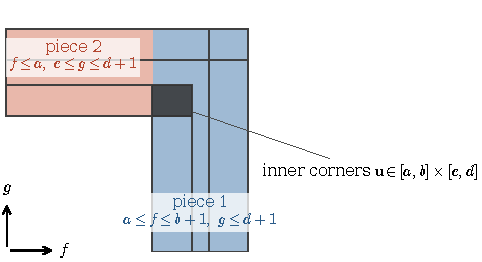
\includegraphics[width=0.62\textwidth]{figures/fig_boxunion.pdf}
\caption{\Cref{lem:boxunion}, drawn in the coordinates $(f,g)$ of the hallway: the union of the hallways $X_j(\bu)$ over all inner corners $\bu$ in the box $[a,b]\times[c,d]$ (dark) is the union of the two shaded convex pieces. Four of the hallways are outlined.}
\label{fig:boxunion}
\end{figure}

\needspace{6\baselineskip}
\begin{lem}\label{lem:boxunion}
Let $a<b$ and $c<d$. Then
\[
\bigcup_{\bu\in[a,b]\times[c,d]}X_j(\bu)\;=\;\widehat{X}_j\;:=\;\{a\le f_j\le b+1,\ g_j\le d+1\}\cup\{f_j\le a,\ c\le g_j\le d+1\}.
\]
\end{lem}

\begin{proof}
A point lies in the first arm of some $X_j(\bu)$ with $\bu\in[a,b]\times[c,d]$ if and only if $a\le f_j\le b+1$ and $g_j\le d+1$, and in the second arm of some such $X_j(\bu)$ if and only if $f_j\le b+1$ and $c\le g_j\le d+1$. The part of the second set with $f_j\ge a$ is contained in the first set.
\end{proof}

For a box $E=\prod_{j}\big([a_j,b_j]\times[c_j,d_j]\big)\subset E_0$ we define
\[
\Gamma(E)=\lamstar\Big(B_W\cap\bigcap_{j=1}^k\widehat{X}_j\Big),
\]
where $\widehat{X}_j$ is formed with $a_j,b_j,c_j,d_j$ as in \cref{lem:boxunion}. For every $\bw\in E$ we have $B_W\cap X(\bw)\subset B_W\cap\bigcap_j\widehat{X}_j$, and therefore
\begin{equation}\label{eq:Gammabound}
\sup_{\bw\in E}\lamstar\big(B_W\cap X(\bw)\big)\le\Gamma(E).
\end{equation}

\subsection{Evaluating \texorpdfstring{$\Gamma(E)$}{Gamma(E)} exactly}\label{sec:exact}

Each set $\widehat{X}_j$ is the union of two closed convex polygonal regions with disjoint interiors, and $B_W$ is a convex polygon. Intersecting $B_W$ with $\widehat{X}_1,\dots,\widehat{X}_k$ one at a time, and splitting every polygon into its intersections with the two pieces of $\widehat{X}_j$, we write $B_W\cap\bigcap_j\widehat{X}_j$ as a union of at most $2^k$ closed convex polygons $P_1,\dots,P_m$ with pairwise disjoint interiors.

To find the connected components, form the \emph{contact graph}: its vertices are the polygons $P_i$, and two of them are joined by an edge if they intersect. The union of the polygons in a connected component of this graph is connected, and unions coming from different components of the graph are disjoint closed sets. So the connected components of $B_W\cap\bigcap_j\widehat{X}_j$ correspond to the components of the contact graph, and the area of each is the sum of the areas of its polygons.

Some polygons may be degenerate, reduced to a segment or a point. They have no area but can connect two other polygons, so they must be kept: discarding them could split a component and make the computed value of $\Gamma(E)$ too small.

The computation is exact if all the numbers involved are rational. Suppose that every angle in $A\cup B$ has rational sine and cosine, that is, $\sin a=p/r$ and $\cos a=q/r$ for a Pythagorean triple $p^2+q^2=r^2$, as for $\arcsin(3/5)$; Kallus and Romik also used such angles \cite[Section~4 and Appendix]{kallusromik2018}. Then all the affine functions $f_j,g_j$ have rational coefficients. If $W$ is rational, the box $E_0$ and every box obtained from it by repeated bisection have rational endpoints. Every vertex of every polygon $P_i$ is then the intersection of two lines with rational coefficients, and every area is rational.

A box $E$ passes the test ``$\Gamma(E)\le T$'' as follows. If $\sum_i\lambda(P_i)\le T$, it passes, since every component has area at most the total. Otherwise the contact graph is computed, and $E$ passes if every component has area at most $T$.

\subsection{Certificates}

\begin{defn}\label{def:certificate}
Let $A$, $B$, $W$ be as in \cref{lem:box} and $T>0$. A \emph{certificate} for the inequality $G(A;B)\le T$ is a finite binary tree whose nodes are boxes in $\R^{2k}$, such that
\begin{enumerate}[label=(\alph*)]
\item the root is the box $E_0$ of \cref{lem:box};
\item the two children of every internal node are the two halves of its box, obtained by bisecting it at the midpoint of one coordinate interval;
\item every leaf $E$ satisfies $\Gamma(E)\le T$.
\end{enumerate}
\end{defn}

\begin{prop}\label{prop:certificate}
If a certificate for $G(A;B)\le T$ exists, then $G(A;B)\le T$.
\end{prop}

\begin{proof}
By induction on the tree, the leaves cover $E_0$. Every $\bw\in E_0$ lies in some leaf $E$, and then $\lamstar(B_W\cap X(\bw))\le\Gamma(E)\le T$ by \eqref{eq:Gammabound}. \Cref{lem:box} completes the proof.
\end{proof}

A certificate is stored as the list of its nodes in preorder. An internal node is recorded as the index of the coordinate that is bisected, and a leaf as the letter \texttt{L}. The boxes themselves are not stored: they are determined by $E_0$ and the sequence of bisections.

\subsection{Finding a certificate}\label{sec:search}

The certificate is produced by a separate search program. At each box it evaluates $\Gamma$ in double-precision floating-point arithmetic. If the value is below $T-10^{-7}$, the box becomes a leaf; otherwise it is bisected along its longest side. The margin $10^{-7}$, and the rule that nearly touching polygons count as touching, make it unlikely that floating-point errors produce a leaf that fails the exact test.

None of these choices affects correctness. A wrong decision by the search can only produce a leaf $E$ with $\Gamma(E)>T$, or a tree of the wrong shape, and the exact check rejects both. In \cite{kallusromik2018} a single program, in exact arithmetic throughout, does both the search and the certification. Separating the two lets the search use fast floating-point arithmetic and keeps the program that must be trusted small.
